\documentclass{article}

\usepackage{amsmath}
\usepackage{amsfonts}
\usepackage{amssymb}
\usepackage{booktabs}
\usepackage{geometry}
\usepackage{graphicx}
\usepackage{tcolorbox}
\usepackage{tikz}
\usepackage{xcolor}

\usetikzlibrary{arrows.meta, calc, patterns, positioning}

\geometry{a4paper, margin=1in}

\newcommand{\notesetup}[1]{
    \title{#1}
    \author{}
    \date{}
}

\newtcolorbox{keyidea}[1]{
    colback=blue!5,
    colframe=blue!45!black,
    title=#1
}

\newtcolorbox{pitfall}[1]{
    colback=red!4,
    colframe=red!55!black,
    title=#1
}


\begin{document}

\notesetup{Thermal Energy, Heat, and Power}
\maketitle

\section{Thermal Energy, Heat, and Temperature}
Many energy transformations in real systems eventually involve thermal effects. To understand this properly, we must distinguish among \textbf{thermal energy}, \textbf{heat}, and \textbf{temperature}.

\begin{itemize}
    \item \textbf{Thermal energy:} the total microscopic kinetic and potential energy of the particles in a substance
    \item \textbf{Heat:} energy transferred from a warmer body or region to a cooler one
    \item \textbf{Temperature:} a measure of the average kinetic energy of the particles in a substance
\end{itemize}

\begin{keyidea}{Important Distinction}
Objects can have the same temperature but different amounts of thermal energy. Heat is not stored inside an object in the same way; heat is the transfer of energy.
\end{keyidea}

\subsection{Comparing Thermal Energy and Temperature}
\begin{itemize}
    \item A large sample of water at $50^\circ \text{C}$ contains more thermal energy than a small sample of water at $50^\circ \text{C}$.
    \item If two samples are at the same temperature, no net heat flows between them.
    \item If two samples have different temperatures, heat flows from the hotter sample to the colder sample.
\end{itemize}

\subsection*{Sample Problem 1: Conceptual Comparison}
\textbf{Problem:} A cup contains $200\,\text{mL}$ of water at $60^\circ \text{C}$. A large pot contains $2.0\,\text{L}$ of water at the same temperature. Which has more thermal energy? Will heat flow if they are mixed?

\textbf{Solution:} The pot contains more thermal energy because it has a much larger mass of water at the same temperature. However, there will be no net heat flow if they are mixed because their temperatures are equal.

\section{Methods of Heat Transfer}
Heat can be transferred in three main ways.

\subsection{Conduction}
Conduction is heat transfer through a material by collisions of particles.

\begin{itemize}
    \item It is most effective in metals.
    \item It explains why a metal spoon becomes hot in a pot of soup.
\end{itemize}

\subsection{Convection}
Convection is heat transfer by the motion of fluid particles.

\begin{itemize}
    \item Warm fluid becomes less dense and rises.
    \item Cooler fluid sinks and replaces it.
    \item This produces a \textbf{convection current}.
\end{itemize}

\subsection{Radiation}
Radiation is heat transfer by electromagnetic waves.

\begin{itemize}
    \item It does not require matter.
    \item This is how energy from the Sun reaches Earth.
\end{itemize}

\begin{figure}[h]
    \centering
    \begin{minipage}{0.31\textwidth}
        \centering
        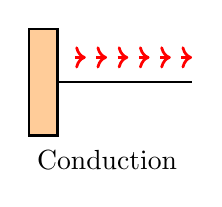
\begin{tikzpicture}[scale=0.9, line width=1pt]
            \draw[fill=orange!40] (-1.1,-0.2) rectangle (-0.7,1.3);
            \draw[thick] (-0.7,0.55) -- (1.2,0.55);
            \foreach \x in {-0.45,-0.15,0.15,0.45,0.75,1.05} {
                \draw[->,red] (\x,0.9) -- (\x+0.15,0.9);
            }
            \node at (0,-0.55) {Conduction};
        \end{tikzpicture}
    \end{minipage}
    \hfill
    \begin{minipage}{0.31\textwidth}
        \centering
        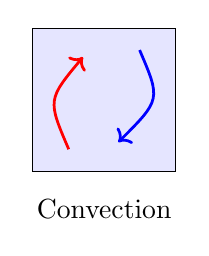
\begin{tikzpicture}[scale=0.9, line width=1pt]
            \draw[thick] (-1,0) rectangle (1,2);
            \fill[blue!10] (-1,0) rectangle (1,2);
            \draw[->,red] (-0.5,0.3) .. controls (-0.8,1.0) .. (-0.3,1.6);
            \draw[->,blue] (0.5,1.7) .. controls (0.8,1.0) .. (0.2,0.4);
            \node at (0,-0.55) {Convection};
        \end{tikzpicture}
    \end{minipage}
    \hfill
    \begin{minipage}{0.31\textwidth}
        \centering
        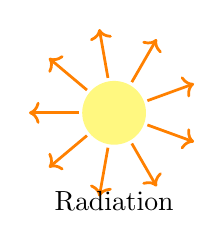
\begin{tikzpicture}[scale=0.9, line width=1pt]
            \fill[yellow!50] (0,0) circle (0.45);
            \foreach \a in {20,60,100,140,180,220,260,300,340} {
                \draw[->,orange] (\a:0.5) -- (\a:1.2);
            }
            \node at (0,-1.25) {Radiation};
        \end{tikzpicture}
    \end{minipage}
    \caption{The three main methods of heat transfer.}
\end{figure}

\subsection*{Sample Problem 2: Identifying the Method}
\textbf{Problem:} Identify the main method of heat transfer in each case:
\begin{enumerate}
    \item A metal pan handle becomes hot.
    \item Warm air rises above a heater.
    \item Sunlight warms the Earth.
\end{enumerate}

\textbf{Solution:}
\begin{enumerate}
    \item conduction
    \item convection
    \item radiation
\end{enumerate}

\section{Calculating Heat Transfer}
Different substances require different amounts of energy to change temperature. This is described by \textbf{specific heat capacity}.

\begin{equation}
    Q = mc\Delta T
\end{equation}

Where:
\begin{itemize}
    \item $Q$ is the heat transferred, measured in joules ($\text{J}$)
    \item $m$ is mass, measured in kilograms ($\text{kg}$)
    \item $c$ is specific heat capacity, measured in $\text{J}/(\text{kg}\cdot^\circ\text{C})$
    \item $\Delta T = T_f - T_i$
\end{itemize}

\begin{keyidea}{Sign Convention}
If an object is heated, $Q$ is positive. If an object cools down, $Q$ is negative.
\end{keyidea}

\subsection*{Sample Problem 3: Heating Water}
\textbf{Problem:} How much heat is needed to raise the temperature of $2.0\,\text{kg}$ of water from $20^\circ \text{C}$ to $75^\circ \text{C}$? Use $c_{\text{water}} = 4.18 \times 10^3\,\text{J}/(\text{kg}\cdot^\circ\text{C})$.

\textbf{Solution:}
\begin{equation*}
    \Delta T = 75 - 20 = 55^\circ \text{C}
\end{equation*}
\begin{equation*}
    Q = mc\Delta T
\end{equation*}
\begin{equation*}
    Q = (2.0)(4.18 \times 10^3)(55)
\end{equation*}
\begin{equation*}
    Q \approx 4.6 \times 10^5\,\text{J}
\end{equation*}

\section{Principle of Heat Exchange}
When heat is transferred between two bodies:

\begin{keyidea}{Principle of Heat Exchange}
The amount of heat lost by the hotter body equals the amount of heat gained by the colder body.
\end{keyidea}

This can be written as
\begin{equation}
    Q_{\text{lost}} + Q_{\text{gained}} = 0
\end{equation}

or, for two materials,
\begin{equation}
    m_1c_1\Delta T_1 + m_2c_2\Delta T_2 = 0
\end{equation}

\subsection*{Sample Problem 4: Mixing Hot and Cold Water}
\textbf{Problem:} A $0.30\,\text{kg}$ sample of hot water at $80^\circ \text{C}$ is mixed with $0.50\,\text{kg}$ of cold water at $20^\circ \text{C}$. Assume no heat is lost to the surroundings. What is the final temperature?

\textbf{Solution:}
Since both samples are water, the specific heat capacity cancels:
\begin{equation*}
    m_1(T_f - 80) + m_2(T_f - 20) = 0
\end{equation*}
\begin{equation*}
    0.30(T_f - 80) + 0.50(T_f - 20) = 0
\end{equation*}
\begin{equation*}
    0.80T_f - 34 = 0
\end{equation*}
\begin{equation*}
    T_f = 42.5^\circ \text{C}
\end{equation*}

\section{Power}
Power describes how fast work is done or how fast energy is transferred.

\begin{equation}
    P = \frac{W}{\Delta t}
    \qquad \text{or} \qquad
    P = \frac{\Delta E}{\Delta t}
\end{equation}

Where:
\begin{itemize}
    \item $P$ is power, measured in watts ($\text{W}$)
    \item $1\,\text{W} = 1\,\text{J/s}$
\end{itemize}

\subsection*{Sample Problem 5: Power from Energy Transfer}
\textbf{Problem:} A cyclist transfers $2.4 \times 10^4\,\text{J}$ of energy in $2.0\,\text{min}$. What is the cyclist's average power?

\textbf{Solution:}
\begin{equation*}
    \Delta t = 2.0\,\text{min} = 120\,\text{s}
\end{equation*}
\begin{equation*}
    P = \frac{\Delta E}{\Delta t}
\end{equation*}
\begin{equation*}
    P = \frac{2.4 \times 10^4}{120} = 2.0 \times 10^2\,\text{W}
\end{equation*}

\subsection*{Sample Problem 6: Power in Climbing}
\textbf{Problem:} A $55\,\text{kg}$ student climbs $3.2\,\text{m}$ vertically in $5.0\,\text{s}$. What is the student's average power?

\textbf{Solution:}
First find the gain in gravitational potential energy:
\begin{equation*}
    \Delta E_g = mgh = (55)(9.8)(3.2) = 1.7 \times 10^3\,\text{J}
\end{equation*}
Then
\begin{equation*}
    P = \frac{\Delta E}{\Delta t} = \frac{1.7 \times 10^3}{5.0}
\end{equation*}
\begin{equation*}
    P \approx 3.4 \times 10^2\,\text{W}
\end{equation*}

\section{Quick Concept Check}
\begin{enumerate}
    \item What is the difference between thermal energy and temperature?
    \item Which heat-transfer method can occur through a vacuum?
    \item If a substance cools down, is $Q$ positive or negative for that substance?
    \item Two machines do the same amount of work, but one does it in less time. Which has more power?
\end{enumerate}

\section{Summary}
\begin{itemize}
    \item Thermal energy, heat, and temperature are related but not identical.
    \item Heat can be transferred by conduction, convection, or radiation.
    \item Heat transfer for a temperature change is found using $Q = mc\Delta T$.
    \item In an isolated heat-exchange problem, $Q_{\text{lost}} + Q_{\text{gained}} = 0$.
    \item Power is the rate of doing work or transferring energy: $P = \frac{W}{\Delta t}$ or $P = \frac{\Delta E}{\Delta t}$.
\end{itemize}

\end{document}
